\begin{center}
    \vspace*{1.5cm}
    {\fontsize{20}{20}\textbf{Snapsvisor}}\\
    \vspace{0.7cm}
    {\fontsize{12}{12}\textit{Om helan själv får välja}}
\end{center}
\addtocwithheader{Snapsvisor}  % Add entry to TOC and set header\noBackground
\noBackground

\newpage
\resetBackground

\begin{textblock*}{3cm}(0.0cm,0.2cm) % {width}(x, y)
    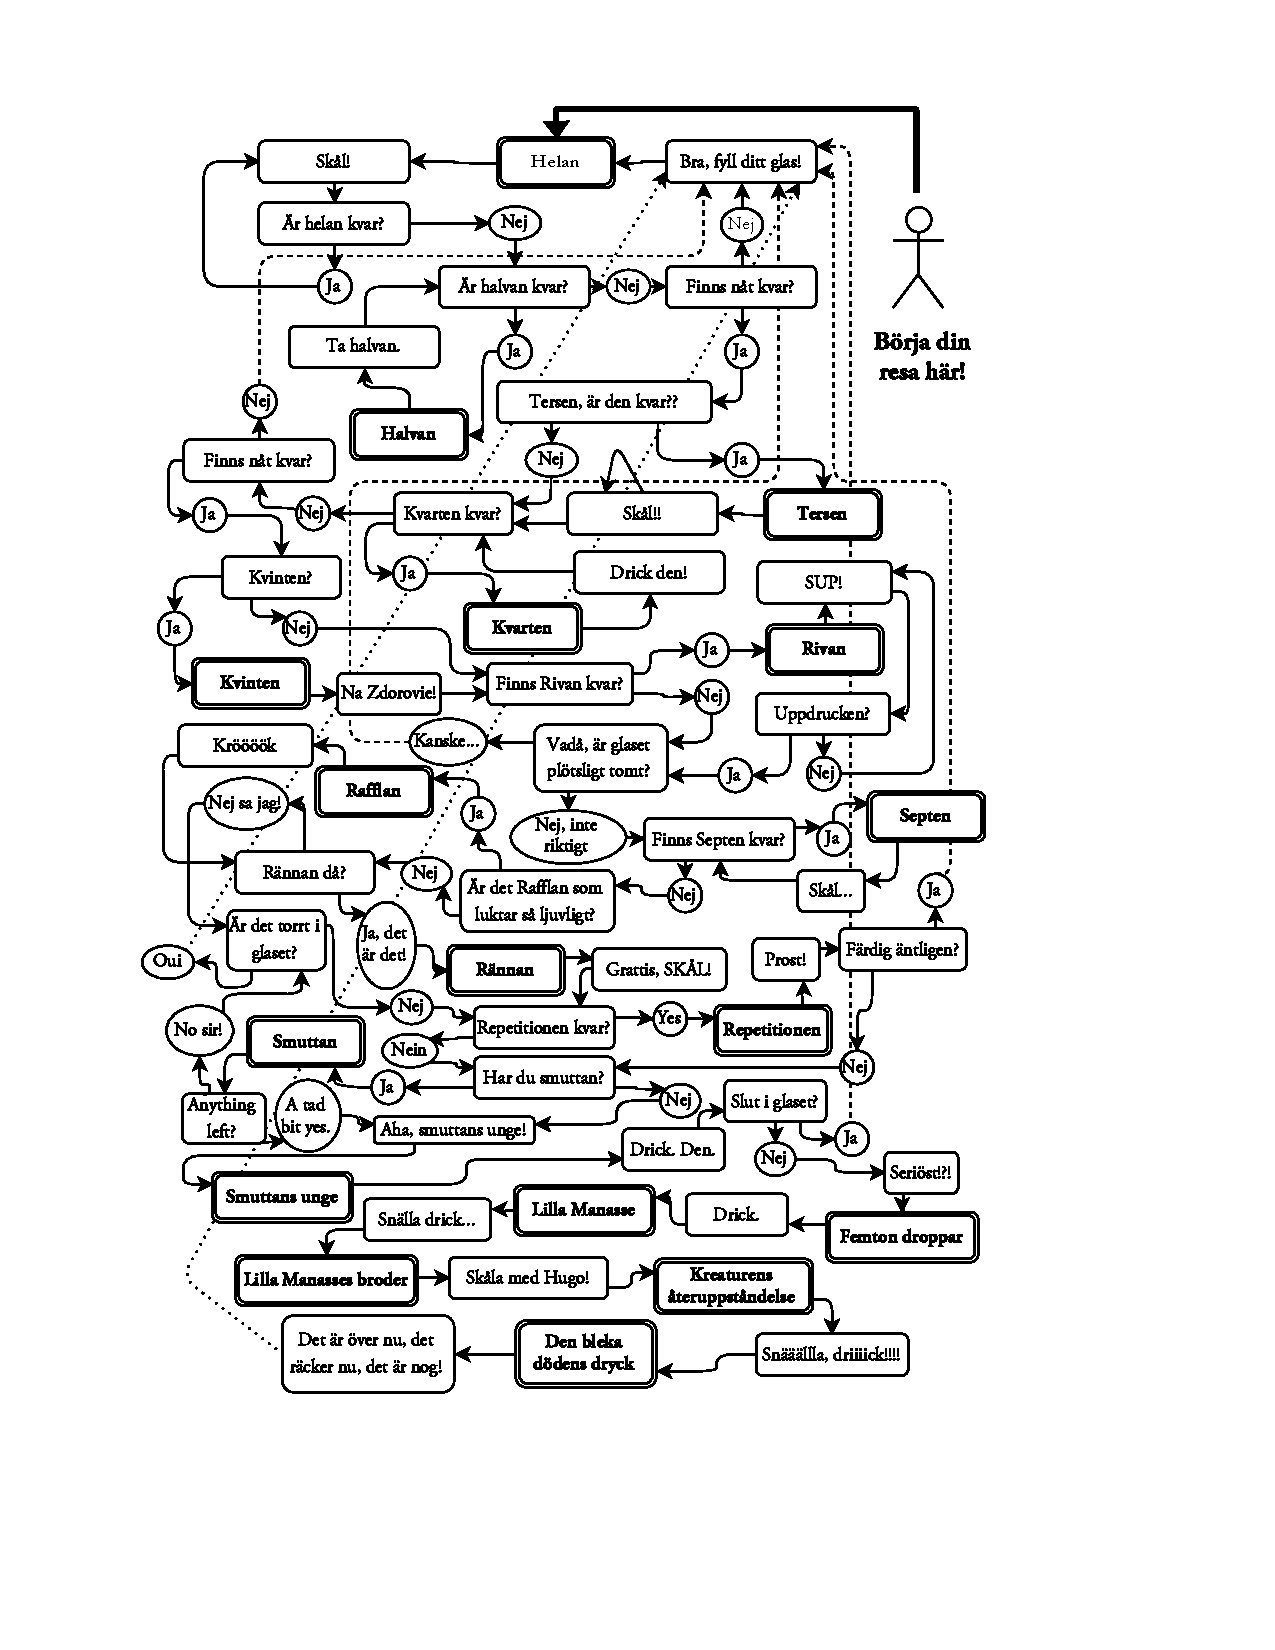
\includegraphics[width=12cm]{./bilder/SupSchema_FINAL_2.pdf}
\end{textblock*}

osynlig text

\vissteduatt{Har du kommit fram till "Den bleka dödens dryck" har du varit \\mycket sparsam. Bra jobbat!}

\newpage

\subsection*{Törsten rasar} 
\index[alfa]{Törsten rasar}
\index[anfa]{Törsten rasar}
\songinfo{Mel: Längtan till landet}

\begin{parse lines}[\noindent]{#1\\}
    Törsten rasar uti våra strupar,
    tungan hänger torr och styv och stel
    Men snart vankas stora, kalla supar,
    var och en får sin beskärda del
    Snapsen kommer, den vi vilja tömma,
    denna nektar lik Olympens saft,
    kommer oss att våra sorger glömma
    Snapsen skänker hälsa, liv och kraft

    Fordom odlade man vindruvsranka,
    av vars frukt man gjorde ädelt vin
    Nu man pressar saften ur en planka,
    doftande av äkta terpentin
    Höj din bägare, O, Broder, yster,
    och låt svenska skogen glida kall,
    ner för strupen och om sen det dig lyster,
    låt oss supa opp en liten tall
\end{parse lines}

\vissteduatt{Visste du att funktionärsposten Macapär infördes efter att sektionen\\köpt sin första Mac?}

\newpage

\begin{parse lines}[\noindent]{#1\\}
    Helan tänder helig eld i själen,
    halvan rosar livet som en sky
    Tersen känns från hjässan ner i hälen,
    kvarten gör oss till en mänska ny
    Låt oss skåla med varann, go' vänner,
    skål för våran levnads glada lopp,
    törstens eld på nytt i strupen bränner
    Leve livet! Skål och botten opp!
\end{parse lines}

\subsection*{Helan går} 
\index[alfa]{Helan går}
\index[anfa]{Helan går}
\songinfo{Kursivt sjunges av sångförman}

\begingroup
\itshape
\noindent Det satt en liten fågel på en gren\\
\noindent och sjöng i furuskogen\\
\noindent Han hade sjungit hela dagen lång,\\
\noindent men dock ej sjungit nog än\\
\noindent Men vad sjöng den lilla fågeln då?\\
\noindent Jo! Han sjöng:\\
\endgroup

\begin{parse lines}[\noindent]{#1\\}
    Helan går,
    sjung hopp faderallan lallan lej,
    Helan går,
    sjung hopp faderallan lej.
    Och den som inte helan tar,
    han heller inte halvan får
    Helan går,
    sjung hopp faderallan lej
\end{parse lines}

\newpage

\subsection*{Samling vid pumpen} 
\index[alfa]{Samling vid pumpen}
\index[anfa]{Samling vid pumpen}
\songinfo{Mel: Hujedamej sån’t barn han var}

\begin{parse lines}[\noindent]{#1\\}
    Samling nu vid pumpen 
    alla ni som dricker vatten 
    Vi som dricker brännvin 
    vi höjer våra glas 
    Vatten ska man ha 
    när man ska vattna i rabatten 
    Brännvin ska man ha 
    när man e på kalas!

\end{parse lines}


\subsection*{Inre dialog} 
\index[alfa]{Inre dialog}
\index[anfa]{Jag vill inte ha}
\songinfo{Mel: An der Schönen Blauen Donau\\
Kursivt sjunges av sångförman}

\textit{Jag vill inte ha} \hfill En nubbe till! \hspace*{15pt} \\
\textit{Jag  mår inte bra} \hfill En nubbe till! \hspace*{15pt} \\
\textit{Om ni ger mig mer} \hfill En nubbe till! \hspace*{15pt} \\
\textit{ser jag er som fler} \hfill En nubbe till! \hspace*{15pt} \\
\textit{Min mage är sjuk} \hfill En nubbe till! \hspace*{15pt} \\
\textit{Min hjärna är mjuk} \hfill En nubbe till! \hspace*{15pt} \\
\\
\textit{Jag kan inte tääänkaaa så braaa}\\
\textit{så jag får väl nubben ta} \hfill HURRA! \hspace*{37pt} 

\vissteduatt{Visste du att rummet Pump heter Pump eftersom fontänens pump\\tidigare stod i det rummet?}

\newpage


\subsection*{Tänk om jag hade lilla nubben} 
\index[alfa]{Tänk om jag hade lilla nubben}
\index[anfa]{uppå ett snöre i halsen}
\songinfo{Mel: Hej, tomtegubbar}

\begin{parse lines}[\noindent]{#1\\}
    Tänk om jag hade lilla nubben
    uppå ett snöre i halsen
    Tänk om jag hade lilla nubben
    uppå ett snöre i halsen
    Jag skulle dra den upp och ner
    så att det kändes som många fler
    Tänk om jag hade lilla nubben
    uppå ett snöre i halsen
\end{parse lines}

\subsection*{Livet är härligt} 
\index[alfa]{Livet är härligt}
\index[anfa]{Livet är härligt}
\songinfo{Mel: Röda kavalleriet \\ Ur Chalmersspexet Katarina II 1959}

\begin{parse lines}[\noindent]{#1\\}
    Livet är härligt!
    Tavarisjtj, vårt liv är härligt!
    Vi alla våra små bekymmer glömmer
    när vi har fått en tår på tanden, SKÅL!

    Tag dig en vodka!
    Tavarisjtj, en liten vodka!
    Glasen i botten vi tillsammans tömmer;
    det kommer mera efter hand

    En SKÅL!
\end{parse lines}

\vissteduatt{Visste du att fler SKÅNSKA snapsvisor finns på sida…}
\newpage


\begin{textblock*}{3cm}(5.3cm,9.5cm) % {width}(x, y)
    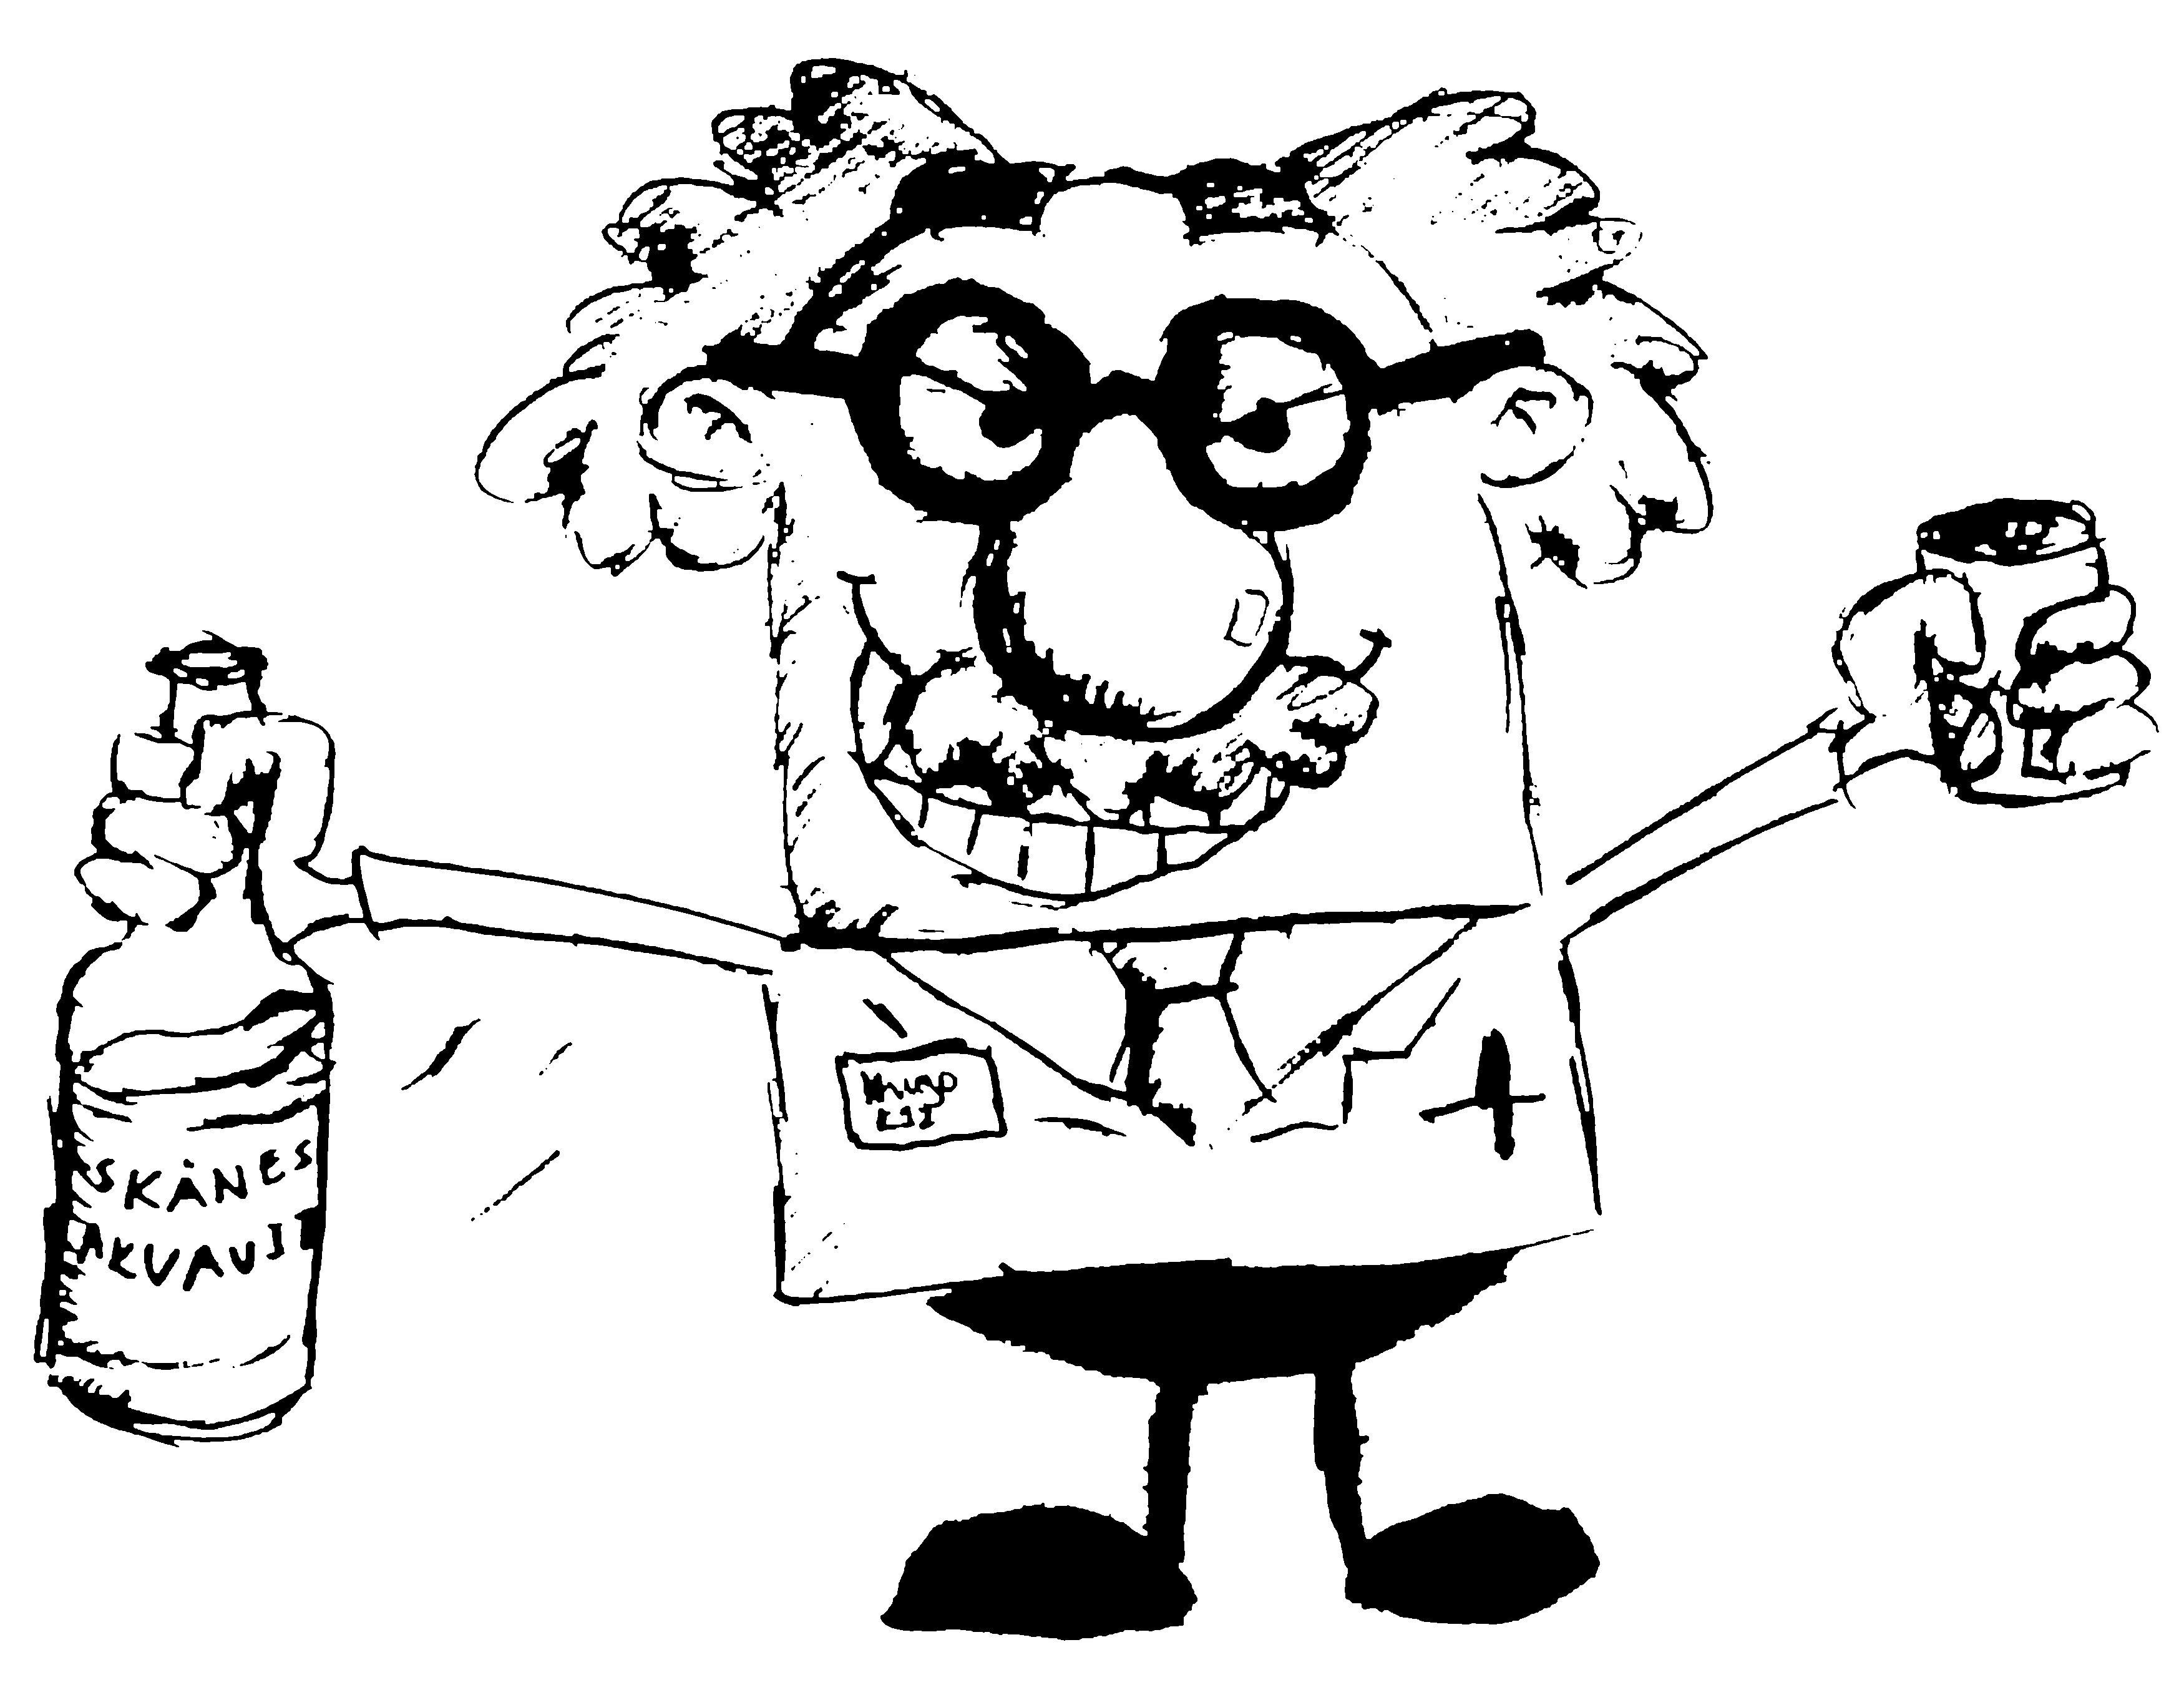
\includegraphics[width=4.5cm]{./bilder/GalenVetenskapsmanTransparent.png}
\end{textblock*}

\subsection*{Det naturliga urvalet} 
\index[alfa]{Det naturliga urvalet}
\index[anfa]{Darwin studerade liv och natur}
\songinfo{Mel: Mors lilla Olle\\
Text: Rolf Malmström}

\begin{parse lines}[\noindent]{#1\\}
    När Darwin studerade liv i natur
    Så fann han att först dör de svagaste djur
    De sämsta bland hjärnceller dör också först
    Så öka din IQ och minska din törst
\end{parse lines}

\subsection*{Lillebror och jag} 
\index[alfa]{Lillebror och jag}
\index[anfa]{Lillebror och jag}
\songinfo{Mel: Måltidssången (refrängen)\\
Lundakarnevalen 1998}

\begin{parse lines}[\noindent]{#1\\}
    Tycker du att snapsen är för stor
    kan du ge en slatt till lillebror
    Både en, både två, både tre, både fem
    och sen blir det fosterhem!
\end{parse lines}


\subsection*{Talteori} 
\index[alfa]{Talteori}
\index[anfa]{1, 2, 75, 6, 7}
\songinfo{Mel: Ritch, ratch}

\begin{parse lines}[\noindent]{#1\\}
    1, 2, 75, 6, 7, 75, 6, 7, 75, 6, 7,
    1, 2, 75, 6, 7, 75, 6, 7, 73,
    107, 103, 102,
    107, 6, 19, 27,
    17, 18, 16, 15,
    13, 19, 14, 17,
    19 16 18 11 
    8 47!
\end{parse lines}

\vissteduatt{Visste du att 1996 började 272 teknologer på E? De var indelade i\\8 klasser med ungefär 32 i varje.}

\newpage

\subsection*{Vikingen} 
\index[alfa]{Vikingen}
\index[anfa]{En viking}
\songinfo{Mel: When Johnny comes marching home\\
Text: Olof Ekdahl\\
E-sektionen Sångarstriden 1981}

\begin{parse lines}[\noindent]{#1\\}
    En viking vill ha livets vann,
    hurra, hurra!
    Den hastigt i mitt svalg försvann,
    hurra, hurra!
    Till kalv, till oxe, till fisk, till fläsk,
    när kärringen bara dricker läsk,
    då vill alla sanna vikingar ha en bäsk

    När vi druckit bäsken slut,
    tragik, tragik!
    Då bäres varje viking ut,
    som lik sig lik
    Och sen, om vi vaknar, vi sjunger en bit,
    sen korkar vi upp Skånes Akvavit
    ||: Skål för alla vikingar som kom hit!:|| 
\end{parse lines}

\subsection*{En gång i månan} 
\index[alfa]{En gång i månan}
\index[anfa]{En gång i månan}
\songinfo{Mel: Mors lilla Olle}

\begin{parse lines}[\noindent]{#1\\}
    En gång i månan är månen full,
    Men aldrig vi sett honom ramla omkull
    Stum av beundran hur mycket han tål,
    Höja vi glasen och dricka hans skål!
\end{parse lines}

\vissteduatt{Visste du att Vikingen skrevs av en E:are? Han heter Olof,\\kallades Öloph, och var sektionens första krögare.}

\newpage

\begin{textblock*}{3cm}(6.7cm,10cm) % {width}(x, y)
    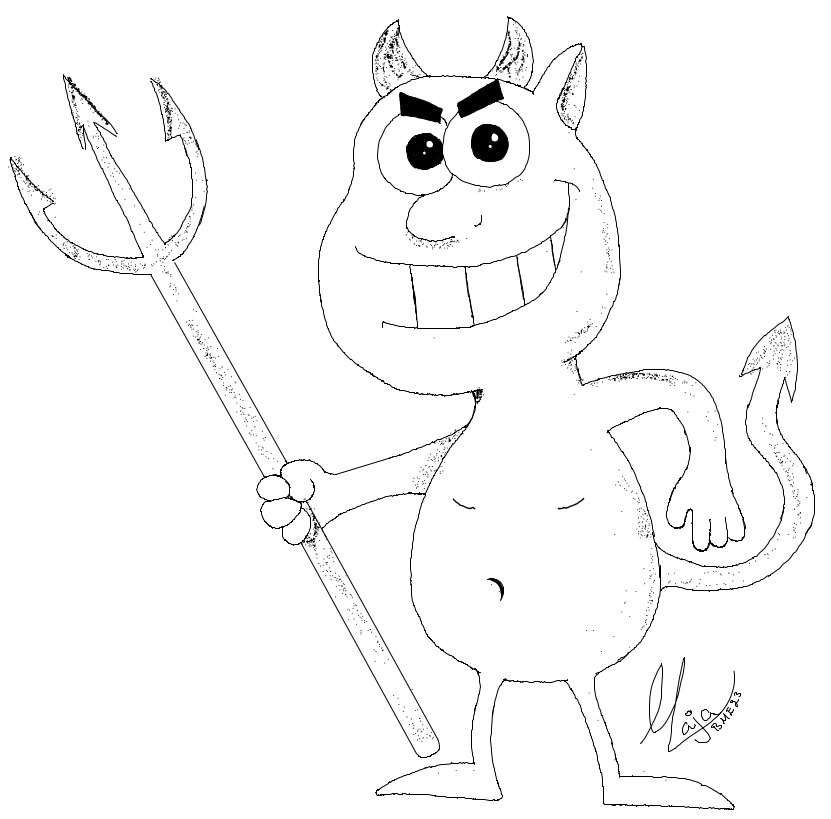
\includegraphics[width=3cm]{./bilder/majas-bilder/devil.png}
\end{textblock*}

\subsection*{Imbelupet} 
\index[alfa]{Imbelupet}
\index[anfa]{Imbelutpet glaset står på bräcklig fot}
\songinfo{Mel: Kors på Idas grav}

\begin{parse lines}[\noindent]{#1\\}
    Imbelupet glaset står på bräcklig fot,
    kalla pilsnerpavor luta sig därmot
    men därnere, miserere,
    uti magens dunkla djup,
    sitter djävulen och väntar på en sup

    uti magens välvda valv, 
    vankar djävulen och ropar på en halv

    uti magen härs och tvärs,
    kilar djävulen och skriker på en ters

    uti magen djup så svart,
    löper djävulen och skränar på en kvart.

    uti magens labyrint,
    irrar djävulen och tjoar på en kvint

    uti magens slingerväxt,
    springer djävulen och skriar på en sext

    uti magen heluppknäppt
    rusar djävulen och vrålar på en sept!

    uti magen an och av
    vankar djävulen och väser på oktav
\end{parse lines}

\vissteduatt{Visste du att E-sektionen var först på LTH att införa ett\\permanent alkoholtillstånd?}

\newpage

\subsection*{Vi skålar för våra vänner} 
\index[alfa]{Vi skålar för våra vänner}
\index[anfa]{Vi skålar för våra vänner}
\songinfo{Mel: Flickan går i ringen}

\begin{parse lines}[\noindent]{#1\\}
    Vi skålar för våra vänner
    och dom som vi känner
    och dom som vi inte känner
    dom skiter vi i!

    Vi skiter i våra vänner
    och dom som vi känner
    och dom som vi inte känner
    dom skålar vi för!
\end{parse lines}

\subsection*{Den som spar den har} 
\index[alfa]{Den som spar den har}
\index[anfa]{Om man bara tar en smutt, smutt, smutt}
\songinfo{Mel: Nu är glada julen slut}

\begin{parse lines}[\noindent]{#1\\}
    Om man bara tar en 
    smutt, smutt, smutt,
    utav denna lilla 
    hutt, hutt, hutt
    har man ganska mycket kvar,
    men se den som spar han har, 
    inte särskilt roligt
\end{parse lines}

\vissteduatt{Visste du att det finns ett svärd på sektionen? Fråga någon i E6 om Krögarsvärdet!}

\newpage

\subsection*{Att fela är mänskligt} 
\index[alfa]{Att fela är mänskligt}
\index[anfa]{Trampa på ett smådjur}
\songinfo{Mel: Prästens lilla kråka\\
Lundakarnevalen 2010}

\begin{parse lines}[\noindent]{#1\\}
    Trampa på ett smådjur,
    slakta gulligt rådjur,
    måste göras rätt försiktigt...

    Gifta sig med släkten,
    stjäla ur kollekten,
    det är fel och det är viktigt!

    ||: Men att sjunga en snutt, och ta sig en hutt
    Det är bara rätt och riktigt! :||
\end{parse lines}

\subsection*{Vår höga skatt} 
\index[alfa]{Vår höga skatt}
\index[anfa]{Vår höga skatt}
\songinfo{Mel: En kulen natt\\
M-sektionen Sångarstriden 2003}

\begin{parse lines}[\noindent]{#1\\}
    Vår höga skatt, skatt, skatt
    Gör att jag korsar
    En bro till främmande, främmande land
    Där spriten forsar
    Och där jag handlade, handlade sprit
    Som jag sen smugglade, smugglade hit
    Så att en su-petti-petti-petti-pett
    Jag kan få ta
    I detta nu!
\end{parse lines}

\vissteduatt{Visste du att det finns ett svärd på sektionen? Fråga någon i KM om Sexmästarsvärdet!}
\newpage

\subsection*{Häll upp en} 
\index[alfa]{Häll upp en}
\index[anfa]{Häll upp en}
\songinfo{Mel: Pilutta dig\\
E-sektionen Sångarstriden 2000}

\begin{parse lines}[\noindent]{#1\\}
    Häll upp en, häll upp en
    Hell, uppenbart att jag är full
    Du får en, du får en,
    du fåren dom har ull
    Så fort man börjat snapsa har,
    man dricker tills dess inget finnes kvar,
    det kanske, det kanske, det kan skena iväg

    Mitt Valhall, mitt Valhall,
    mitt val - Hallands, det gör så gott
    I magen, I magen, i magen min är flott
    Finess och stil är mitt gebit,
    jag biter aldrig av när jag får sprit,
    jag tar en, jag tar en, jag tar en jäkel till!
\end{parse lines}


\subsection*{Mjölkade en ko} 
\index[alfa]{Mjölkade en ko}
\index[anfa]{Mjölkade en ko}
\songinfo{Mel: Jag fångade en räv}

\begin{parse lines}[\noindent]{#1\\}
    Jag mjölkade en ko idag 
    Men när jag såg juvret 
    Då hade jag nog tagit fel 
    För gladast var nog tjuren
\end{parse lines}

\newpage

\begin{textblock*}{3cm}(6.7cm,1.0cm) % {width}(x, y)
    
\includegraphics[width=1.4cm]{./bilder/humla.png}
\end{textblock*}
\begin{textblock*}{3cm}(7.2cm,2.2cm) % {width}(x, y)
    
\includegraphics[width=3cm]{./bilder/humla_signerad.png}
\end{textblock*}
\begin{textblock*}{3cm}(6.9cm,4.9cm) % {width}(x, y)
    
\includegraphics[width=1.6cm]{./bilder/humla.png}
\end{textblock*}
\begin{textblock*}{3cm}(8.0cm,5.9cm) % {width}(x, y)
    
\includegraphics[width=2cm]{./bilder/humla.png}
\end{textblock*}
\begin{textblock*}{3cm}(6.0cm,9.0cm) % {width}(x, y)
    
\includegraphics[width=1.4cm]{./bilder/humla.png}
\end{textblock*}

\subsection*{Humlorna} 
\index[alfa]{Humlorna}
\index[anfa]{Humlorna}
\songinfo{Mel: Här kommer Karl-Alfred boy}

\begin{parse lines}[\noindent]{#1\\}
    ||: Vi äro små humlor vi bzz, bzz :||
    Vi äro små humlor som tar oss en geting
    Vi äro små humlor vi bzz, bzz

    ||: Vi äro små fiskar vi blubb, blubb :||
    Vi äro små fiskar som tar oss en kallsup
    Vi äro små fiskar vi blubb, blubb

    ||: Vi äro små änglar vi flax, flax :||
    Vi äro små änglar som tar oss en Djävel
    Vi äro små änglar vi flax, flax
\end{parse lines}

\subsection*{Stopp en stund} 
\index[alfa]{Stopp en stund}
\index[anfa]{Stopp en stund}
\songinfo{Mel: Räven raskar över isen}

\begin{parse lines}[\noindent]{#1\\}
    Stopp en stund med skratt och pratet,
    kniv och gaffel lägg på fatet
    Seden är, att så här,
    man handskas med destilatet

    Man lyfter glaset med höger hand,
    och trycker läpparna mot dess rand
    Man dricker ur, och grinar sur,
    och väntar på resultatet
\end{parse lines}


\newpage

\begin{textblock*}{3cm}(5.5cm,2.8cm) % {width}(x, y)
    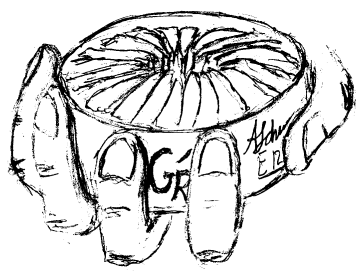
\includegraphics[width=4.5cm]{./bilder/snus.png}
\end{textblock*}


\subsection*{Jag har aldrig varit på snusen} 
\index[alfa]{Jag har aldrig varit på snusen}
\index[anfa]{Jag har aldrig varit på snusen}
\songinfo{Mel: O så saligt att få vandra}

\begin{parse lines}[\noindent]{#1\\}
    Jag har aldrig vatt på snusen,
    aldrig rökat en cigarr - halleluja!
    Mina dygder äro tusen,
    inga syndiga laster jag har

    Jag har aldrig sett nå't naket,
    inte ens ett litet nyfött barn
    Mina blickar går mot taket,
    därmed undgår jag frestarens garn

    ||: Halleluja - halleluja! :||

    Bachus spelar på gitarren,
    Satan spelar på sitt handklaver
    Alla djävlar dansar tango,
    säg vad kan man väl önska sig mer?

    Jo, att alla bäckar vore brännvin,
    stadsparksdammen full av bayerskt öl,
    konjak i varenda rännsten
    och punsch i varendaste pöl

    Och mera öl…
    Vomera öl…
\end{parse lines}

\newpage


\subsection*{Jag har aldrig varit på UB} 
\index[alfa]{Jag har aldrig varit på UB}
\index[anfa]{Jag har aldrig varit på UB}
\songinfo{Mel: O så saligt att få vandra\\
E-sektionen Sångarstriden 2009}

\begin{parse lines}[\noindent]{#1\\}
    Jag har aldrig varit på UB,
    aldrig pluggat på Café Athen,
    aldrig skurit upp en snubbe,
    kan ej skilja artär från ven

    Jag har aldrig börjat klockan 9,
    eller slutat 14:32
    I AF-borgen går jag vilse,
    för jag går på LTH

    Dom har aldrig var't på ön Ön,
    aldrig målat Väg och Vattens spik
    Aldrig haft det stora nöjet,
    att få somna till Böijers logik

    Dom har aldrig vunnit en Regatta,
    eller festat i en skitig overall
    Aldrig däckat bakom Lophtet,
    för dom går ej på LTH

    E kan j-omega och Ohms lag
    F och Nano fattar kvantfysik
    Eko, eko, eko, eko,
    eko, eko med akvavit

\end{parse lines}

\newpage

\begin{parse lines}[\noindent]{#1\\}

    I och M kan ragga på kemister
    Data knackar på sin kära linuxkod
    Inga här är humanister,
    för vi är alla LTH

    I och M kan ragga på kemister
    Data knarkar på sin kära linuxkod
    Mardrömmar om humanister,
    drömmer alla på LTH
\end{parse lines}

\subsection*{Dricka upp} 
\index[alfa]{Dricka upp}
\index[anfa]{Visst kan man dricka långsamt}
\songinfo{Mel: Här kommer Pippi Långstrump}

\begin{parse lines}[\noindent]{#1\\}
    Visst kan man dricka långsamt,
    hälla opp eller ner eller ingen ta
    Visst kan man dricka långsamt,
    men det tänker inte jag!
\end{parse lines}

\subsection*{The BASIC song} 
\index[alfa]{The BASIC song}
\index[anfa]{LET oss nu fatta}
\songinfo{Mel: Mors lilla Olle}

\begin{parse lines}[\noindent]{#1\\}
    \textcolor{gray}{\texttt{10}} \texttt{LET} oss nu fatta i våra glas 
    \textcolor{gray}{\texttt{20}} \texttt{INPUT} en klunk utav det som där has 
    \textcolor{gray}{\texttt{30}} \texttt{IF} du fått nog \texttt{THEN} till \texttt{50} min vän 
    \textcolor{gray}{\texttt{40}} \texttt{ELSE GOTO}-baka till \texttt{10} igen 
    \textcolor{gray}{\texttt{50}} \texttt{END}
\end{parse lines}


\vissteduatt{Visste du att innan pandemin skrevs alla programmeringstentor\\
 med papper och penna?}
\newpage



\begin{textblock*}{3cm}(5.2cm,7.5 cm) % {width}(x, y)
    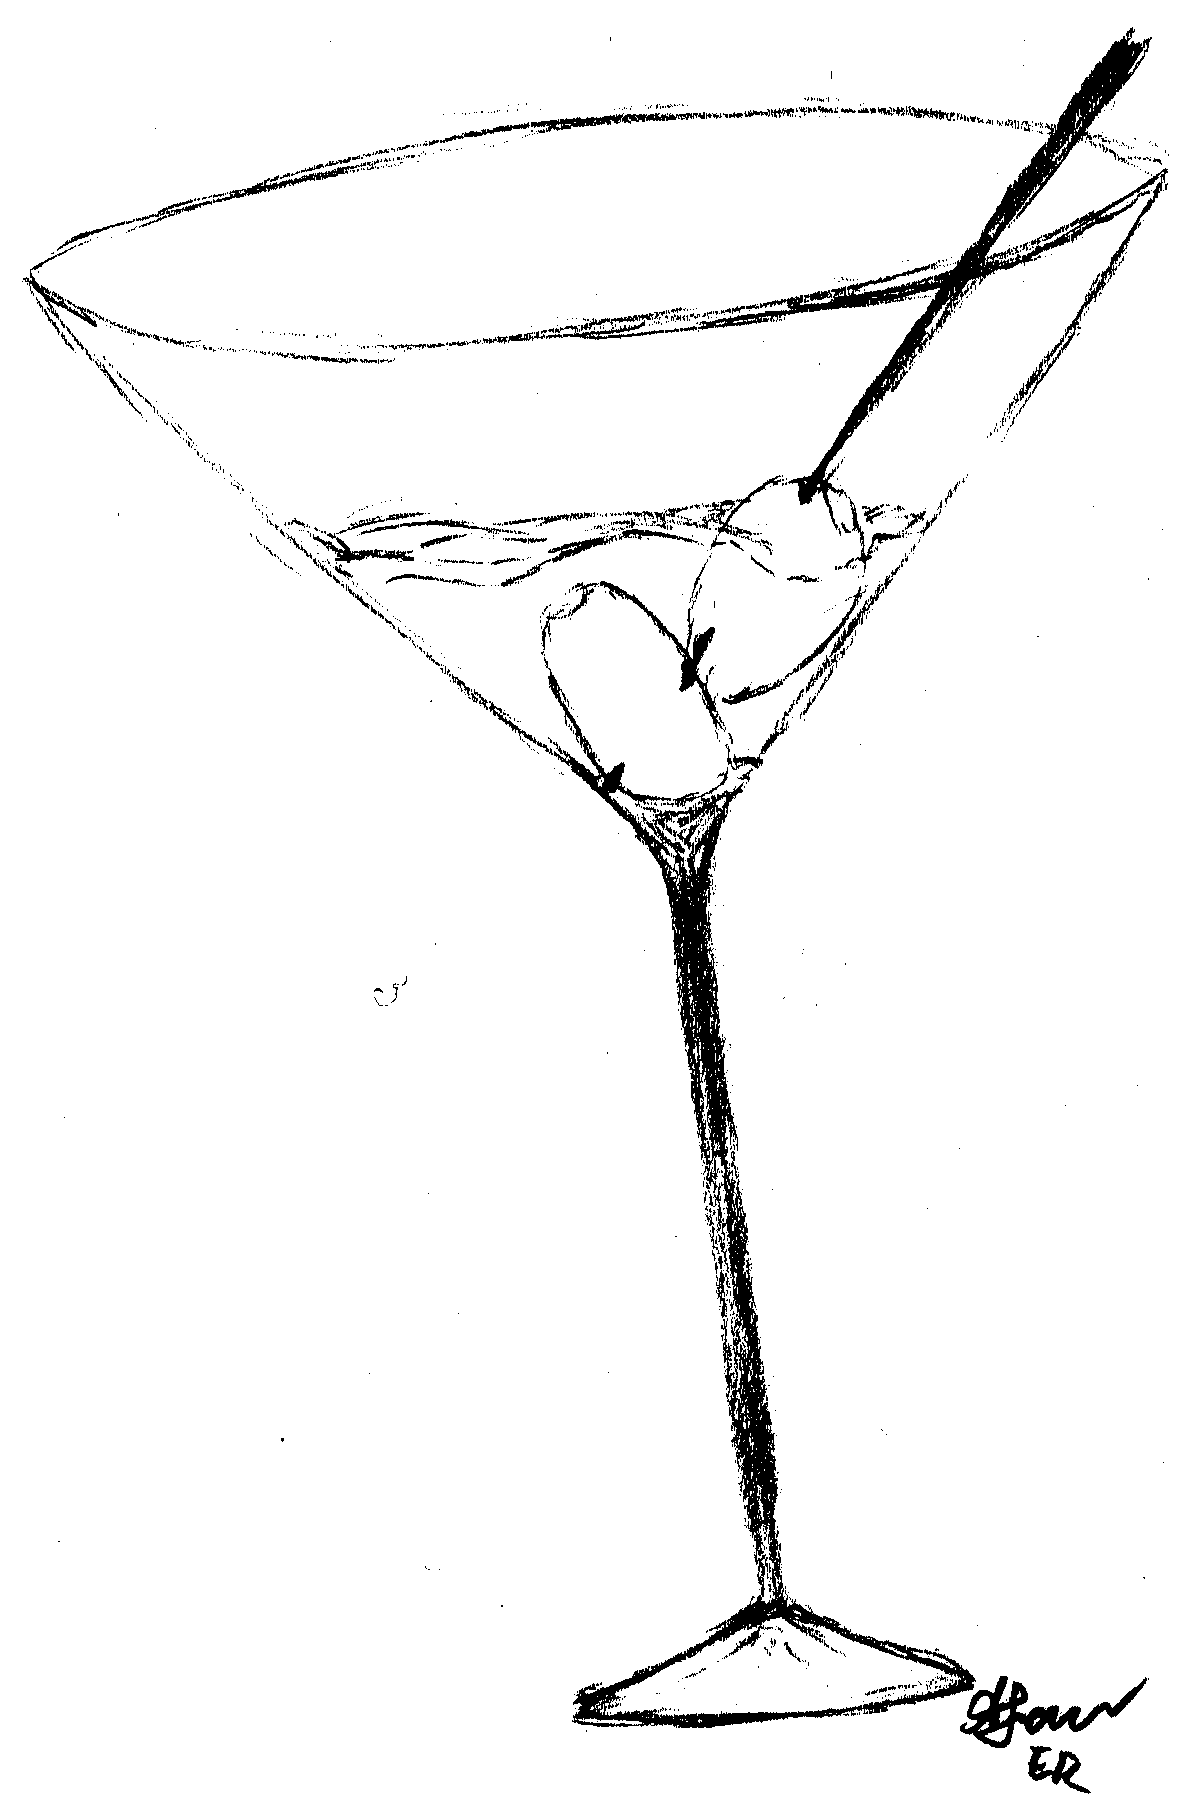
\includegraphics[width=4.0cm]{./bilder/ub.png}
\end{textblock*}




\subsection*{De som är nyktra} 
\index[alfa]{De som är nyktra}
\index[anfa]{De som är nyktra}
\songinfo{Mel: Du är den ende}

\begin{parse lines}[\noindent]{#1\\}
    De som är nyktra 
    har inte så roli't,
    de har bara ansvar 
    och inte nå't tjolitt-
    an-lej-faderulla 
    men vi som är fulla 
    vi har bara kul nästan jämt

    Det sägs att en män'ska 
    kan va' utan brännvin,
    det stämmer måhända 
    men se blott på den min
    som pryder en absolutist, 
    den e' jävligt trist
    därför så sjunger vi nu:

    De som är nyktra 
    har inte så roli't,
    de har bara ansvar 
    och inte nå't tjolitt-
    an-lej-faderulla 
    men vi som är fulla 
    vi har bara kul nästan jämt
\end{parse lines}



\newpage


\subsection*{Vi som är nyktra} 
\index[alfa]{Vi som är nyktra}
\index[anfa]{Vi som är nyktra}
\songinfo{Mel: Du är den ende}

\begin{parse lines}[\noindent]{#1\\}
    Vi som är nyktra
    vi har faktiskt roligt.
    Jo visst har vi ansvar,
    men minst lika
    tjolittanlej faderulla
    som ni som är fulla
    som tror ni har kul nästan jämt

    Men tänk då efter
    uppå dagen efter
    de dagar med fester,
    med smärtsamma rester
    utav eran hjärna,
    nog tycker ni gärna.
    Att va nykterist är nåt visst

    Vi som är nyktra,
    vi har bara roligt
    Imorrn kan vi
    återigen ha det
    tjolittanlej faderulla,
    men ni som är fulla
    aj, aj, aj, det är väl för trist
\end{parse lines}



\newpage

\subsection*{Mera brännvin} 
\index[alfa]{Mera brännvin}
\index[anfa]{Mera brännvin i glasen}
\songinfo{Mel: Internationalen}

\begin{parse lines}[\noindent]{#1\\}
    Mera brännvin i glasen,
    mera glas på vårt bord,
    mera bord på kalasen,
    mer kalas på vår jord.

    Mera jordar med måne,
    mera månar i mars,
    mera marscher till Skåne,
    mera Skåne, Gud bevars, bevars, bevars!
\end{parse lines}

\subsection*{En kulen snaps} 
\index[alfa]{En kulen snaps}
\index[anfa]{En kulen snaps}
\songinfo{Mel: En kulen natt}

\begin{parse lines}[\noindent]{#1\\}
    En kulen snaps, snaps, snaps
    Den står vid faten
    Om jag nu vågade, vågade
    ta den före maten
    Men värden håller ett jäkla långt tal
    Kanske min snaps inte längre hålls sval
    Så ner i djupetetetet
    Den snapsen slank
    Menns den var kall!
\end{parse lines}

\vissteduatt{Visste du att det finns en finsk version av Mera Brännvin?\\Se Internationella visor!}

\newpage


\subsection*{Feministvikingen} 
\index[alfa]{Feministvikingen}
\index[anfa]{Feministvikingen}
\songinfo{Mel: When Johnny Comes Marching Home}


\begin{parse lines}[\noindent]{#1\\}
    En viking viker tvätten själv
    Hurra hurra!
    Ordet "viking" kommer sig därav, jaha!
    Föräldraledigheten delas exakt
    När vikingen sina barn har lagt
    Då är vikingens fru ute på jakt

    En viking vill ha livets vann
    Hurra hurra!
    Men på sig själv han lägger band,
    Jaha, vad bra!
    Mjödet prioriteras sist,
    Tvätta och städa blir aldrig trist
    För våran viking, han är feminist
\end{parse lines}

\subsection*{Änglahund} 
\index[alfa]{Änglahund}
\index[anfa]{Det står en hund}
\songinfo{Mel: Marseljäsen
\\ V-sektionen sångarstriden 1991}

\begin{parse lines}[\noindent]{#1\\}
    Det står en hund på fjärde våningen 
    och den tänker hoppa ner!
    BANZAI!
    Det var en japanesisk självmordhund 
    och den hoppar aldrig mer!
\end{parse lines}



\newpage

\subsection*{Nu dags taga sig en snaps strax} 
\index[alfa]{Nu dags taga sig en snaps strax}
\index[anfa]{Nu dags taga sig en snaps strax}
\songinfo{Mel: Can-Can}

\begin{parse lines}[\noindent]{#1\\}
    Nu dags
    taga sig en snaps strax,
    som din kropp tar opp och
    låter rinna ner.
    Och ger dig smak för flera

    Ditt liv,
    blott ett tidsfördriv, du 
    kastar ner en kask och 
    lever glatt och ler,
    när fler du ser.

    Med sill,
    eller vad du vill till,
    håll din strupe våt, åt
    Bacchus ge din själ,
    han vill dig bara väl.

    Så skjut 
    först en kort salut ut
    nu tar sången slut, trut.
    Gapa, svälj och njut!
\end{parse lines}


\newpage

tom sida

\newpage